\documentclass[10pt,xcolor={table,dvipsnames},t]{beamer}

\usetheme{Madrid} 
\usecolortheme{default} 
\setbeamertemplate{footline}{
  \leavevmode%
  \hbox{%
    \begin{beamercolorbox}[wd=.8\paperwidth,ht=2.5ex,dp=1ex,left]{author in head/foot}%
      \hspace{1em}\insertshorttitle
    \end{beamercolorbox}%
    \begin{beamercolorbox}[wd=.2\paperwidth,ht=2.5ex,dp=1ex,right]{date in head/foot}%
      \insertframenumber{} / \inserttotalframenumber\hspace{1em}
    \end{beamercolorbox}}%
  \vskip0pt%
}
\usepackage{graphicx}
\usepackage{amsmath}
\usepackage{amssymb}
\usepackage{siunitx}

%  link color to be cyanish blue
\definecolor{myblue}{RGB}{0, 153, 204}
\usepackage{hyperref}
\hypersetup{
    colorlinks=true,
    linkcolor=myblue,
    filecolor=magenta,      
    urlcolor=myblue,
    pdftitle={Theremin},
    pdfpagemode=FullScreen,
    }
\sisetup{per-mode=symbol}

\title[Theremin]{Theremin Design and Simulation}
\author{Krish Pandya (2023102026) \and Vaibhav Wadhwani (2023102058)}
\institute{IIITH}
\date{} 
\begin{document}

\begin{frame}
  \titlepage
\end{frame}

\begin{frame}{Outline}
  \tableofcontents
\end{frame}

\section{Introduction}

\begin{frame}{Introduction to Theremin}
\begin{itemize}
    \item An electronic musical instrument played without physical contact.
    \item Invented by L\'{e}on Theremin around 1920.
    \item Uses two antennas to control pitch and volume based on hand proximity.
    \item Operates on the principle of heterodyning: mixing two high-frequency signals to produce an audible difference frequency.
    \item \textbf{Why heterodyning instead of generating audio directly?}
    \begin{itemize}
        \item LC oscillators are more stable and precise at higher frequencies (100s of kHz to MHz).
        \item Producing stable low-frequency (20 Hz–20 kHz) tones directly with LC circuits is inefficient and inaccurate.
        \item Heterodyning down to audio gives better control and tunability.
    \end{itemize}
    \item The player's hands act as the grounded plates of variable capacitors, influencing the frequency of oscillators.
\end{itemize}
\end{frame}

\section{Working Principles}

\begin{frame}{Working Principle of a Theremin}
\begin{itemize}
    \item \textbf{Capacitive Sensing}: The player's hands near the antennas alter the capacitance in oscillator circuits.
    \item \textbf{Oscillators}:
    \begin{itemize}
        \item \textbf{Variable Frequency Oscillator (VFO)}: Frequency changes based on hand distance from the pitch antenna.
        \item \textbf{Fixed Frequency Oscillator (FFO)}: Generates a constant reference frequency.
    \end{itemize}
    \item \textbf{Heterodyning (Mixing)}: The VFO and FFO signals are combined (mixed). The output contains sum and difference frequencies.
    \item \textbf{Filtering}: Low-pass filtering isolates the difference frequency ($f_{VFO} - f_{FFO}$), which falls within the audible range.
    \item \textbf{Volume Control}: Typically uses a separate oscillator circuit affected by the volume antenna to control the final output amplitude. We are using a different approach. Potentiometer ( Standard Volume Knobs)
\end{itemize}
\end{frame}

\section{Circuit Overview}

\begin{frame}{Circuit Overview}
\begin{figure}
    \centering
    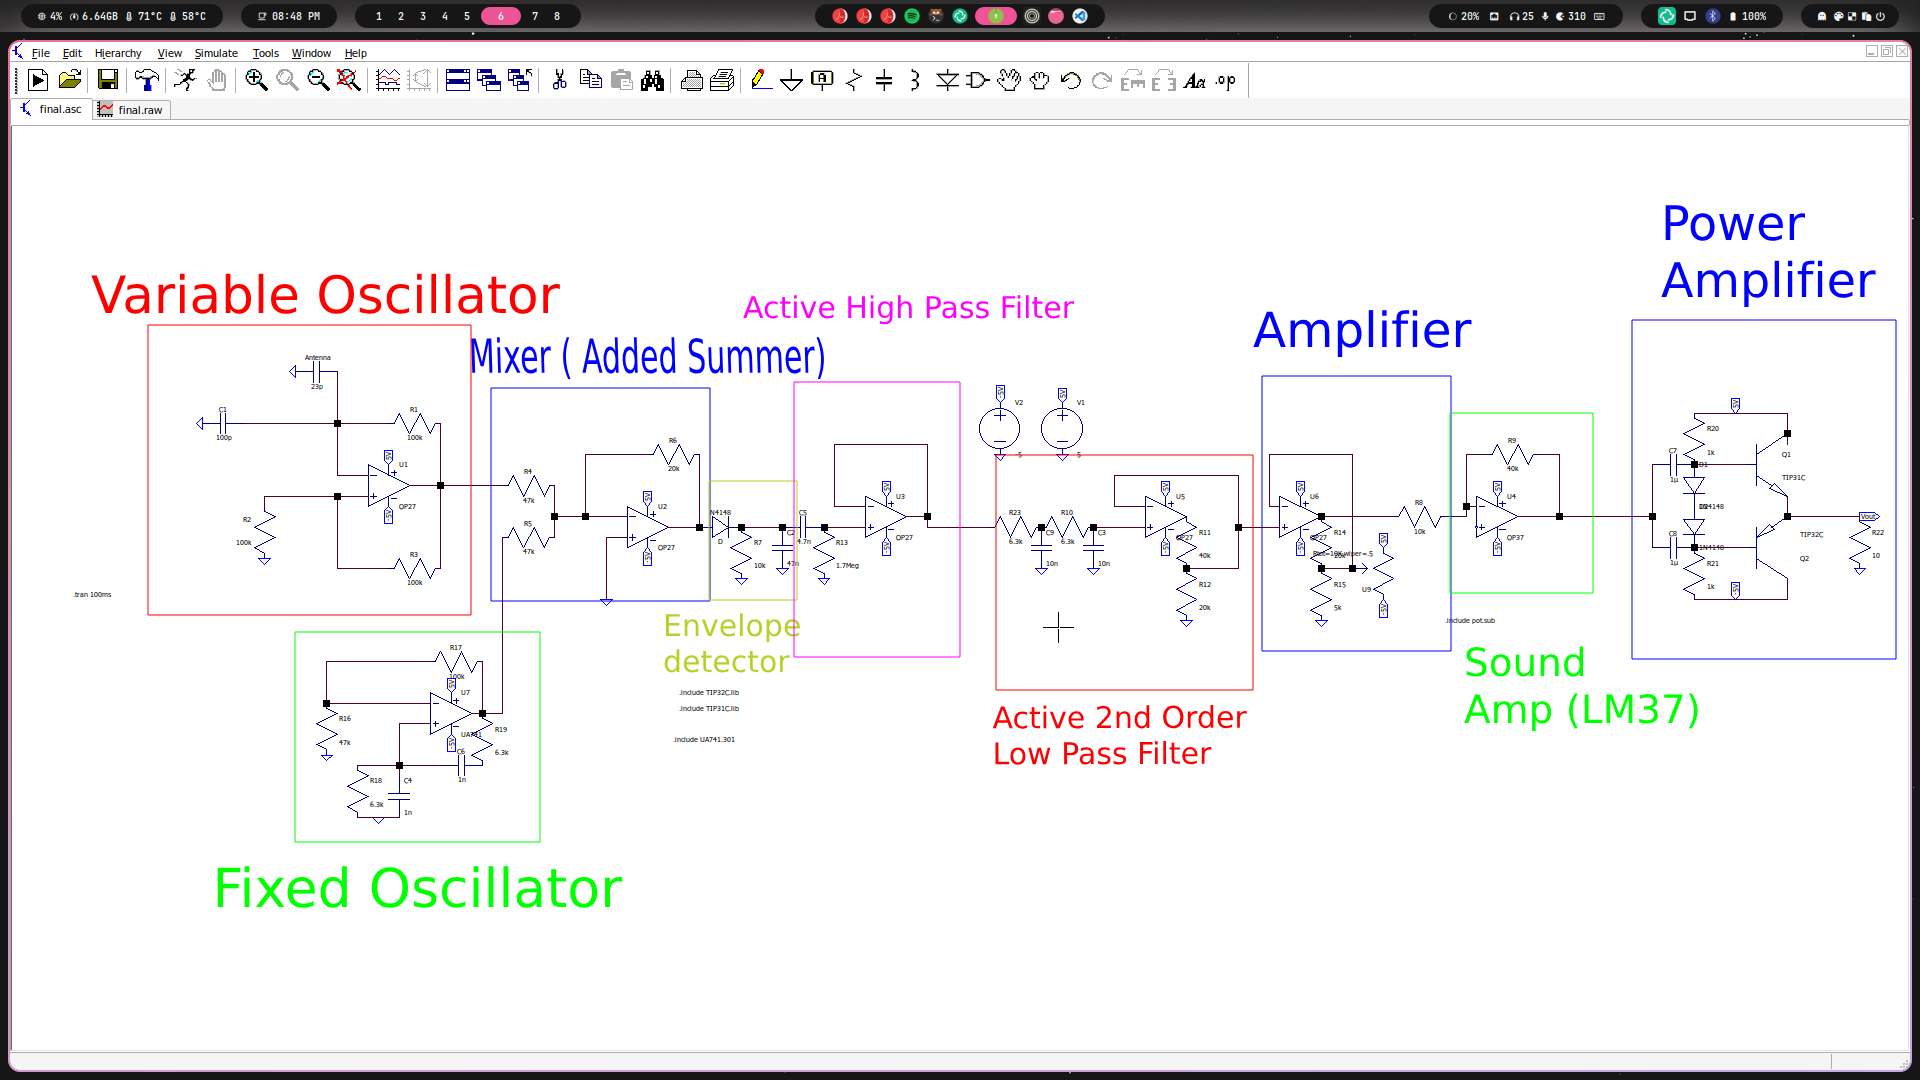
\includegraphics[width=0.95\textwidth, height=0.7\textheight, keepaspectratio]{theremin_circuit.png}
    \caption{Simulated Theremin Circuit Schematic (LTSpice)}
    \label{fig:circuit_overview}
\end{figure}
\vspace{-1em}
\scriptsize
\begin{itemize}
    \item The circuit consists of several stages: Variable Oscillator, Fixed Oscillator, Mixer/Summer, Filters, Amplifiers, and Power Amplifier.
    \item Operational Amplifiers (Op-Amps) like OP27, UA741, OP37 are used extensively.
    \item Power is supplied via a dual rail (+5V / -5V).
\end{itemize}
\end{frame}

\section{Physical Circuit Overview}

\begin{frame}{Physical Circuit Overview}
\begin{figure}
    \centering
    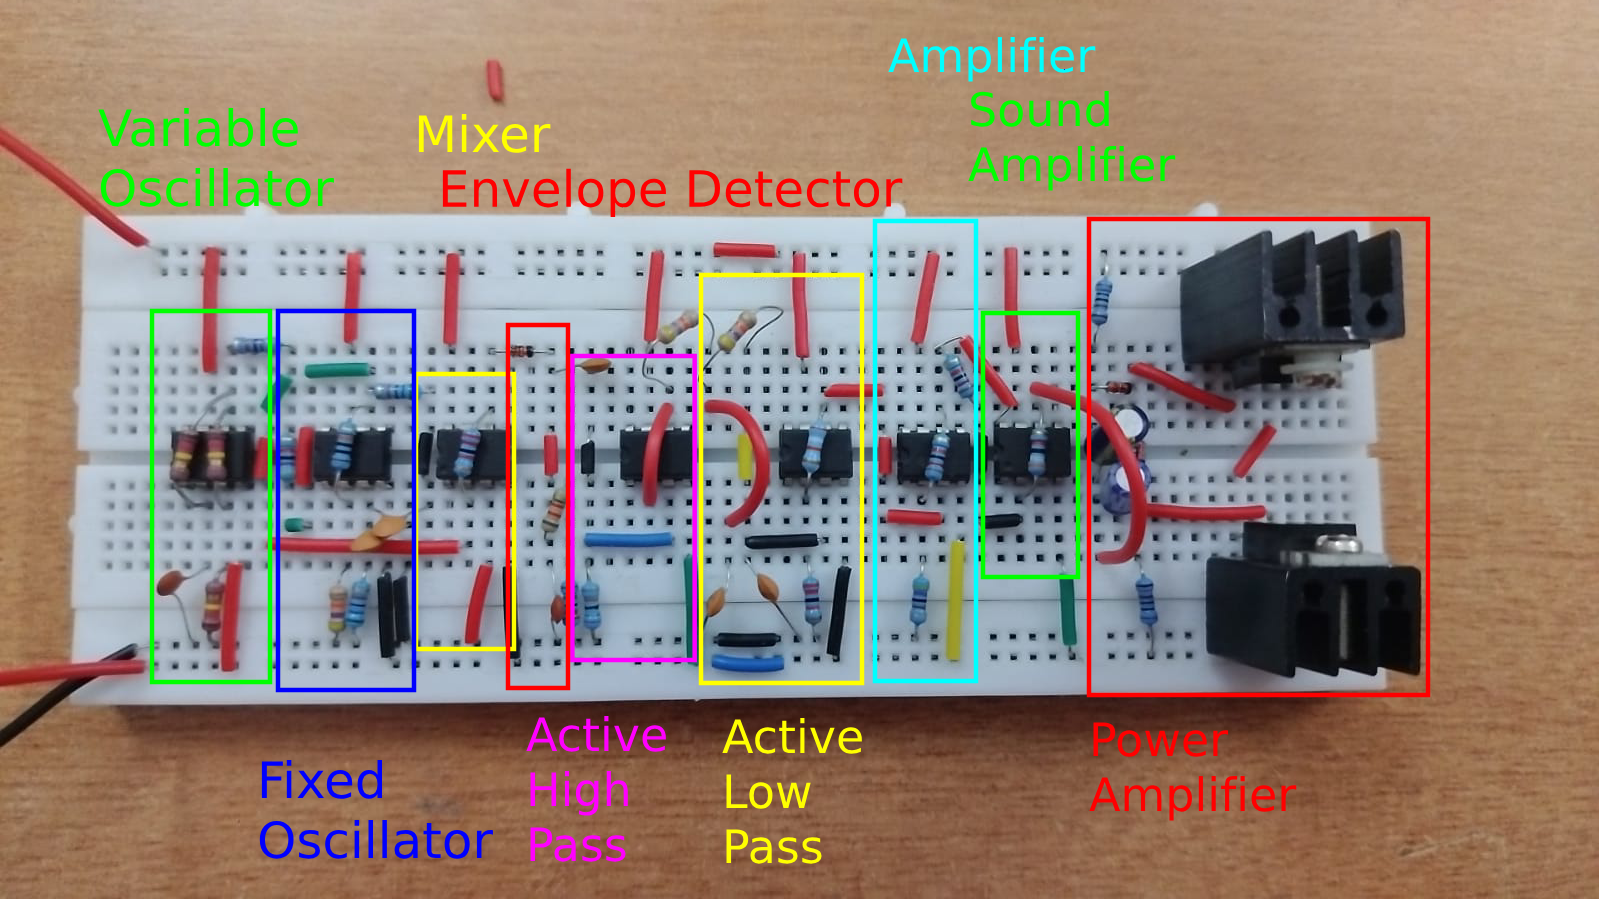
\includegraphics[width=0.95\textwidth, height=0.7\textheight, keepaspectratio]{physical_cirucit.png}
    \caption{Theremin Circuit Schematic (Physical)}
    \label{fig:physical_circuit_overview}
\end{figure}
\vspace{-1em}
\end{frame}


\section{Variable Oscillator (Pitch Control)}

\begin{frame}{Variable Oscillator (Pitch Control)}
\begin{itemize}
    \item \textbf{Function}: Generates a frequency signal that changes based on hand capacitance near the 'Antenna'.
    \item \textbf{Topology}: Op-Amp based oscillator (OP27). Likely a relaxation type oscillator. \href{https://circuitdigest.com/tutorial/relaxation-oscillator-using-op-amp}{Reference}
      \item \textbf{Key Components}:
    \begin{itemize}
        \item U1: OP27 Op-Amp
        \item R1, R2, R3: \SI{100}{\kilo\ohm} resistors (biasing and feedback)
        \item C1: \SI{100}{\pico\farad} capacitor
        \item Antenna: \SI{23}{\pico\farad} capacitor (base capacitance, hand adds variable capacitance in parallel)
    \end{itemize}
    \item \textbf{Operation}: The total capacitance at the input influences the oscillation frequency. As the hand moves closer, capacitance increases, typically lowering the frequency.  
    \item \textbf{Note}: You will hear high frequency oscillation when hand is getting closer because of the heterodyning effect. As this frequency decreases , the difference in frequencies increases and you will hear a high pitch sound.
    \item \textbf{Calculation}:
\end{itemize}
\end{frame}

\begin{itemize}
    \item \textbf{Oscillation Frequency ($f_o$)}:
    \begin{align*}
      f_o = \frac{1}{2R C ln\frac{1+k}{1-k}} \approx \frac{1}{2(120k)(175p)\cdot ln(3)} \approx \SI{21.92}{\kilo\hertz}
      \\\\ \text{where} k = \frac{R2}{R1+R2}  
    \end{align*}
    \item \textbf{Total Capacitance ($C_{total}$)}:
    \begin{align*}
    C_{total} = C_{base} + C_{hand} = 60p + C_{hand}
    \end{align*}
    \item As $C_{hand}$ increases, $f_o$ decreases.
    \item \textbf{Capacitance Change}:
    \begin{align*}
    C_{hand} = \frac{C_{base}}{(1 - \frac{f_o}{f_{max}})} - C_{base}
    \end{align*}
    % result from physical circuits
    \begin{figure}
        \centering
        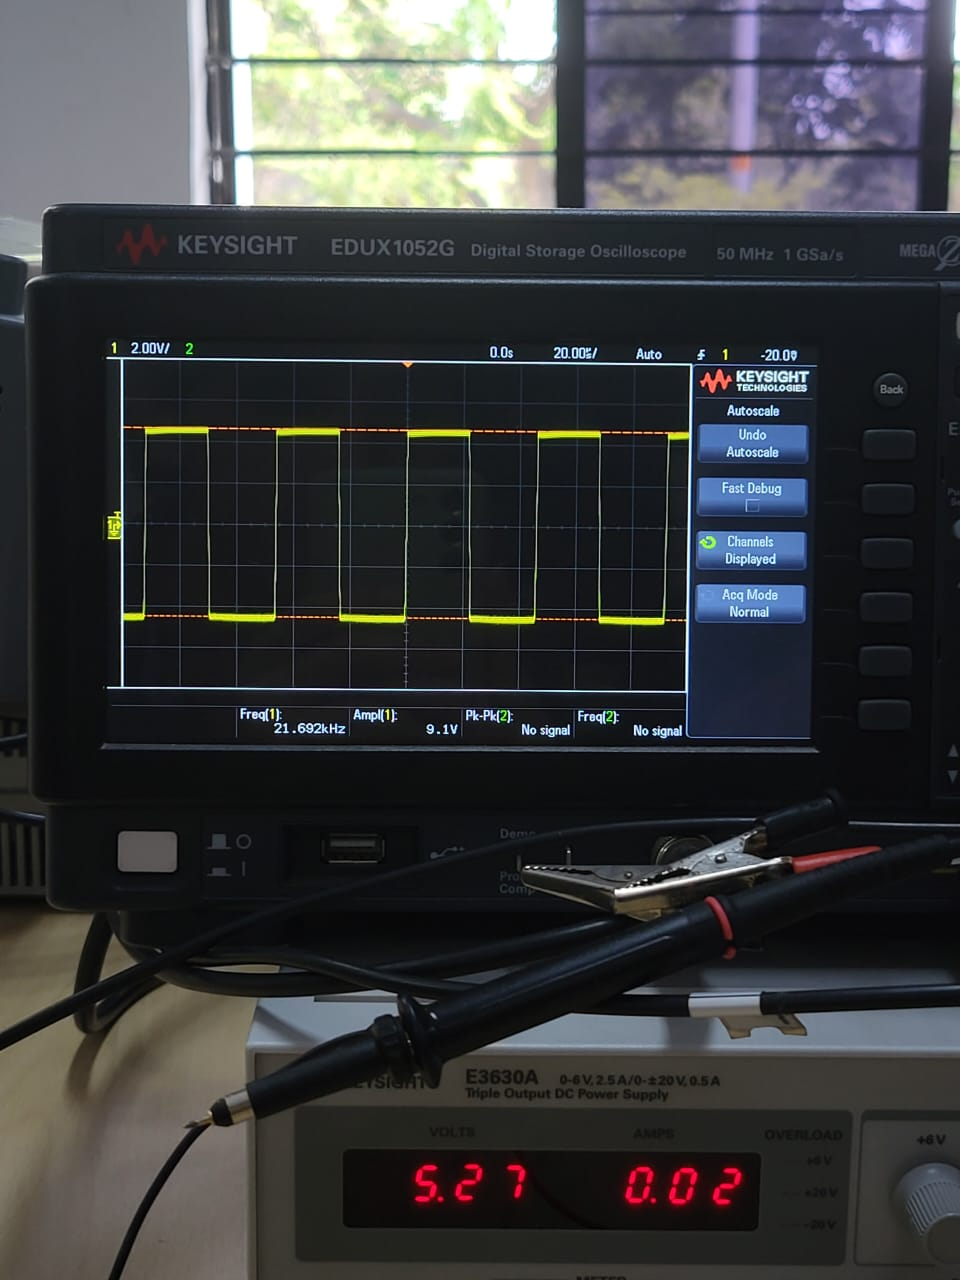
\includegraphics[width=0.8\textwidth]{variable.jpeg}
        \caption{Variable Oscillator Output}
        \label{fig:Variable_Oscillator}
    \end{figure}     
\end{itemize}

\section{Fixed Oscillator (Reference)}

\begin{frame}{Fixed Oscillator (Reference)}
\begin{itemize}
    \item \textbf{Function}: Generates a stable reference frequency for heterodyning.
    \item \textbf{Topology}: Wien Bridge Oscillator using U7 (UA741 Op-Amp).
    \item \textbf{Key Components}:
    \begin{itemize}
        \item U7: UA741 Op-Amp
        \item Frequency Determining Network: R18=\SI{6.3}{\kilo\ohm}, C4=\SI{1}{\nano\farad}, R19=\SI{6.3}{\kilo\ohm}, C6=\SI{1}{\nano\farad}
        \item Gain Setting Network: R16=\SI{47}{\kilo\ohm}, R17=\SI{100}{\kilo\ohm}
    \end{itemize}
\end{itemize}
\end{frame}

\begin{frame}{Fixed Oscillator (Reference) - Calculations}
\begin{itemize}
    \item \textbf{Calculation}:
    \begin{itemize}
        \item Oscillation Frequency ($f_o$):
        \begin{align*}
        f_o = \frac{1}{2\pi RC} \approx \SI{23.26}{\kilo\hertz}
        \end{align*}
        \item Required Gain ($A_v$): $A_v \approx 2.13$
    \end{itemize}
\end{itemize}
\end{frame}

\begin{frame}{Fixed Oscillator (Reference) - Output}
\begin{itemize}
    \item \textbf{Note}: The frequency (\SI{\sim 25}{\kilo\hertz}) is lower than typical Theremin RF oscillators.But because our relaxation oscillator is working at around 21KHz, we are using this frequency to get a better sound.
\end{itemize}
\begin{figure}
    \centering
    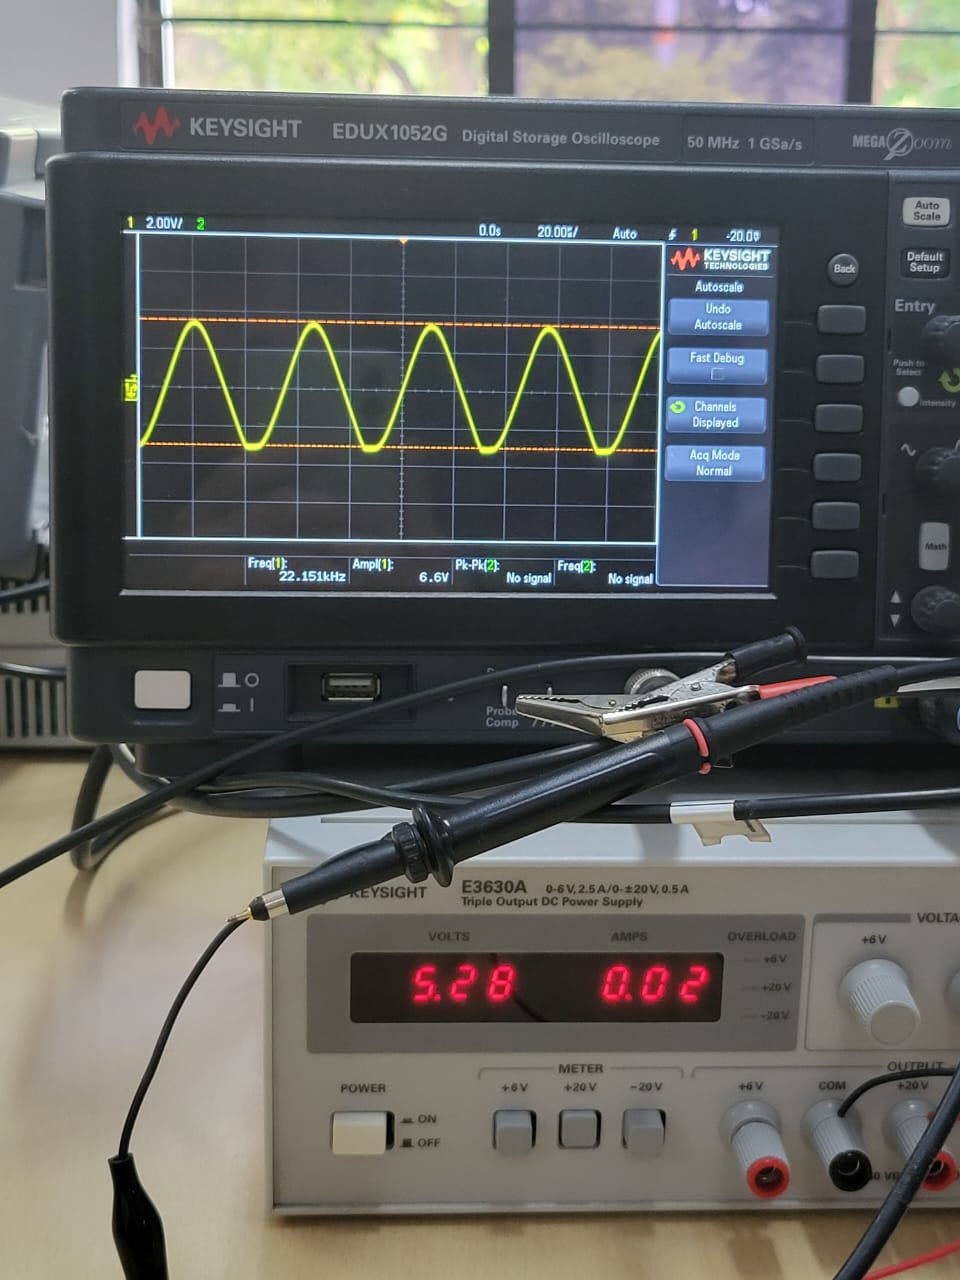
\includegraphics[height=0.9 \textwidth]{fixed.jpeg}
    \caption{Fixed Oscillator Output}
    \label{fig:Fixed_Oscillator}
\end{figure}
\end{frame}

\section{Mixer (Summing Amplifier)}

\begin{frame}{Mixer (Summing Amplifier)}
\begin{itemize}
    \item \textbf{Function}: Combines the signals from the Variable and Fixed Oscillators.
    \item \textbf{Topology}: Inverting Summing Amplifier using U2 (OP27).
    \item \textbf{Key Components}:
    \begin{itemize}
        \item U2: OP27 Op-Amp
        \item Input Resistors: R4=\SI{47}{\kilo\ohm} (from Variable Osc.), R5=\SI{47}{\kilo\ohm} (from Fixed Osc.)
        \item Feedback Resistor: R6=\SI{20}{\kilo\ohm}
    \end{itemize}
    \item \textbf{Calculation}:
    \begin{itemize}
        \item Gain for each input: $G = -\frac{R_f}{R_{in}} \approx -0.426$
        \item Output Voltage: $V_{out} = -0.426 \times (V_{VarOsc} + V_{FixedOsc})$
    \end{itemize}
\end{itemize}
\end{frame}

\section{Filtering Stages}

\begin{frame}{Envelope Detector}
\begin{itemize}
    \item \textbf{Components}: Diode D (1N4148), R7 (\SI{10}{\kilo\ohm}), C2 (\SI{47}{\nano\farad})
    \item \textbf{Function}: Half-wave rectification followed by RC low-pass filtering. Extracts the envelope of the signal from the mixer. \href{https://www.winlab.rutgers.edu/~crose/322_html/envelope_detector.html}{Reference}
    \item \textbf{Time Constant}: $\tau = R7 \times C2 = \SI{0.47}{\milli\second}$
    \item \textbf{Cutoff Freq.}: $f_c \approx 1/(2\pi\tau) \approx \SI{339}{\hertz}$
    \item \textbf{Note}: Placement after mixer is unconventional for standard Theremin volume control. And is intentional design choice to suppress the DC offset created by the envelope detector.
\end{itemize}

\end{frame}

\section{Envelope Detector Output}
\begin{frame}{Envelope Detector Output}
\begin{figure}
    \centering
    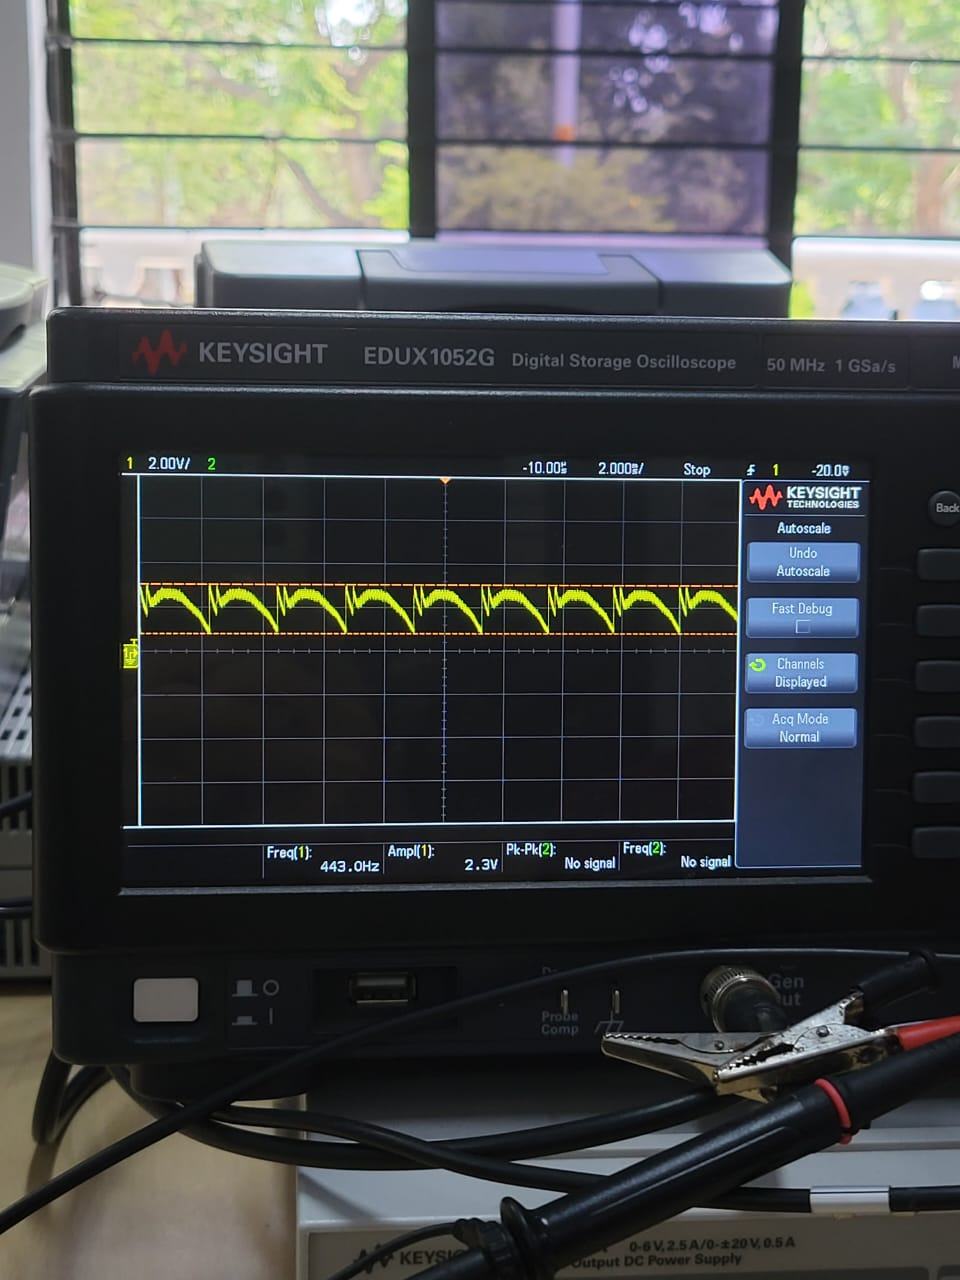
\includegraphics[height=0.8\textwidth]{envelopeoutput.jpeg}
    \caption{Envelope Detector Output}
\end{figure}

\end{frame}

\begin{frame}{Active Filters}
\textbf{Active High Pass Filter}
\begin{itemize}
    \item \textbf{Components}: U3 (OP27), C5 (\SI{4.7}{\nano\farad}), R13 (\SI{1.7}{\mega\ohm})
    \item \textbf{Topology}: 1st order HPF using Op-Amp buffer.
    \item \textbf{Function}: Removes DC offset and very low frequencies.
    \item \textbf{Note}: The cutoff frequency is set to allow audio frequencies while blocking DC. This is important because of the envelope detector output.
    \item \textbf{Cutoff Freq.}: $f_c = \frac{1}{2\pi R13 C5} \approx \SI{19.9}{\hertz}$
\end{itemize}
\vspace{1em}
\textbf{Active 2nd Order Low Pass Filter}
\begin{itemize}
    \item \textbf{Components}: U5 (OP27), R10 (\SI{6.3}{\kilo\ohm}), R11 (\SI{40}{\kilo\ohm}), R12 (\SI{20}{\kilo\ohm}), C3 (\SI{10}{\nano\farad}),R23 (\SI{6.3}{\kilo\ohm}) , C9 (\SI{10}{\nano\farad})
    \item \textbf{Topology}: 2nd order LPF using Op-Amp Feedback for amplification.
    \item \textbf{Function}: Removes high-frequency components above the desired audio range.
    \item \textbf{Cutoff Freq.}: $f_c = \frac{1}{2\pi R10 C3} \approx \SI{2.53}{\kilo\hertz}$
    \item \textbf{Gain}: $G_{DC} = 1 + \frac{R11}{R12} = 1 + \frac{40}{20} = 3$
\end{itemize}



\end{frame}



\section{High Pass Output}
\begin{frame}{High Pass Output}
\begin{figure}
    \centering
    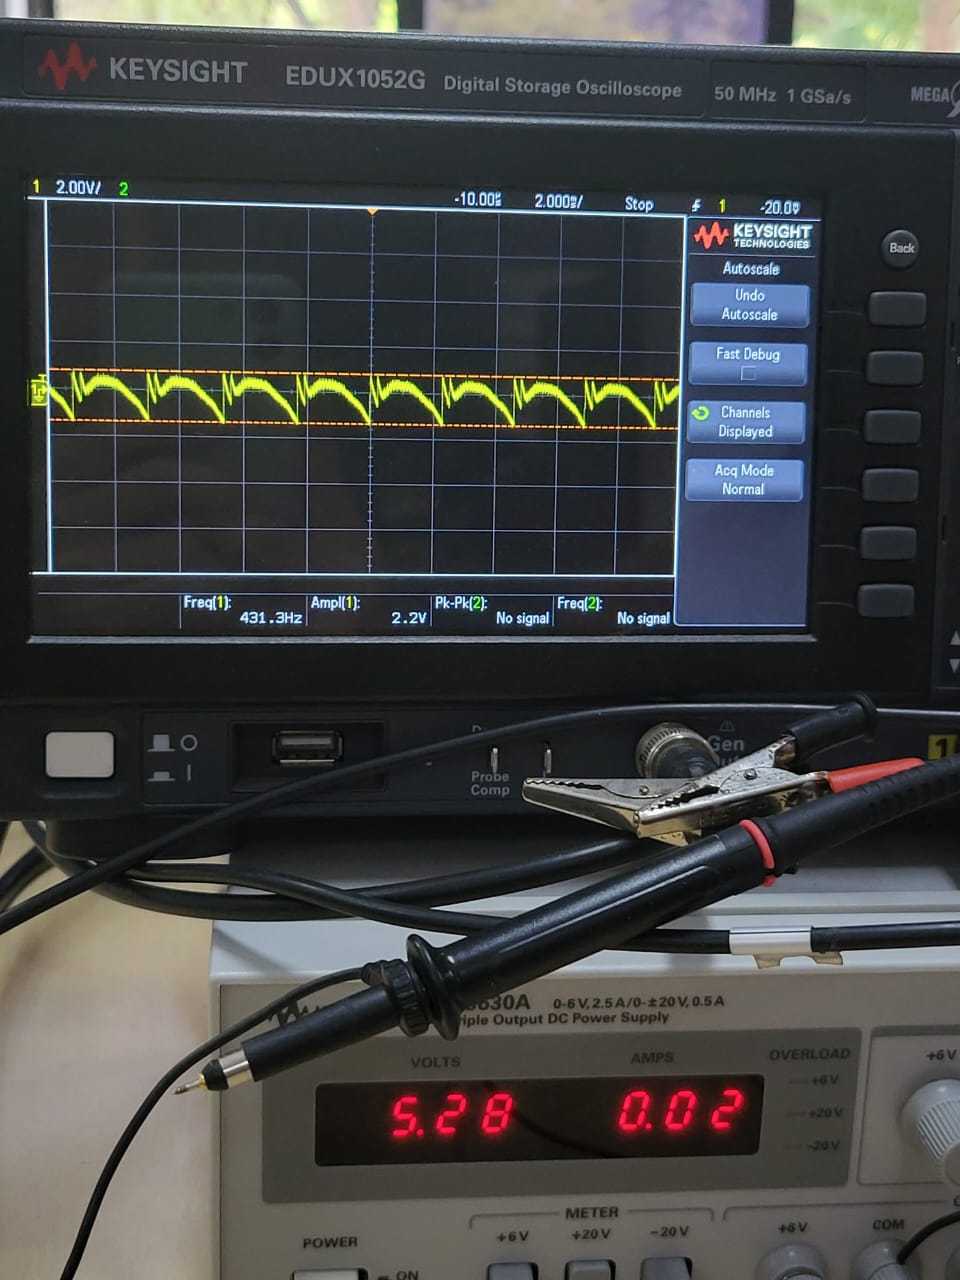
\includegraphics[width=0.8\textwidth]{highpass.jpeg}
    \caption{Filter Stage Output}
\end{figure}
\end{frame}

\section{Amplifier Stages}

\begin{frame}{Pre-Amplifier / Volume Control}
\begin{itemize}
    \item \textbf{Components}: U6 (OP27),  R14 (\SI{20}{\kilo\ohm}), R15 (\SI{5}{\kilo\ohm}), U9 (Potentiometer, \SI{10}{\kilo\ohm})
    \item \textbf{Topology}: Non-inverting amplifier with adjustable gain via potentiometer U9.
    \item \textbf{Function}: Amplifies the filtered audio signal and provides user volume control.
    \item \textbf{Gain Range}: $A_v = 1 + \frac{R14}{R15 + R_{U9}}$
    \begin{itemize}
        \item Min Gain (U9=\SI{10}{\kilo\ohm}): $A_v = 2.33$
        \item Max Gain (U9=\SI{0}{\kilo\ohm}): $A_v = 5$
    \end{itemize}
\end{itemize}
\vspace{1em}
\textbf{Sound Amplifier}
\begin{itemize}
    \item \textbf{Components}: U4 (OP37), R9 (\SI{40}{\kilo\ohm}), R8 (\SI{10}{\kilo\ohm}),
    \item \textbf{Topology}: Sound amplifier using OP37.
    \item \textbf{Function}: Further amplifies the audio signal to drive the power amplifier.
    \item \textbf{Gain}: $G = -\frac{R9}{R8} = -4$
\end{itemize}
\end{frame}

\section{Power Amplifier}

\begin{frame}{Power Amplifier}
\begin{itemize}
    \item \textbf{Function}: Boosts the signal power to drive a low-impedance load like a speaker (R22).
    \item \textbf{Topology}: Class AB Push-Pull Output Stage.
    \item \textbf{Key Components}:
    \begin{itemize}
        \item Q1: TIP31C (NPN BJT)
        \item Q2: TIP32C (PNP BJT Complementary Pair)
        \item D1, D2: 1N4148 diodes for biasing (reduce crossover distortion)
        \item R20, R21: \SI{1}{\kilo\ohm} base current limiting/biasing resistors
        \item C7, C8: \SI{1}{\micro\farad} bypass/filtering capacitors
        \item R22: \SI{10}{\ohm} Load Resistor (representing speaker)
    \end{itemize}
    \item \textbf{Operation}: Q1 conducts for positive signal swings, Q2 conducts for negative swings. Diodes provide a small forward bias to minimize the "dead zone" near zero crossings.
\end{itemize}
\end{frame}

\section{Power Supply}
\begin{frame}{Power Supply Requirements}
\begin{itemize}
    \item \textbf{Dual Rail Supply}:
    \begin{itemize}
        \item Voltage: $\pm \SI{5}{\volt}$ DC (V1 and V2)
        \item Current: \SI{10}{\milli\ampere} to \SI{100}{\milli\ampere}
    \end{itemize}
    
    \item \textbf{Battery Implementation}:
    \begin{itemize}
        \item Two 9V batteries connected in series
        \item Center tap connection between batteries
        \item Voltage regulation:
            \begin{itemize}
                \item LM7805 for +5V regulation
                \item LM7905 for -5V regulation
            \end{itemize}
    \end{itemize}
    
    \item \textbf{Power Consumption}:
    \begin{itemize}
        \item Op-Amps: Low power consumption
        \item BJT stages: Moderate current draw
        \item Total power typically under \SI{3}{\watt}
    \end{itemize}
\end{itemize}
\end{frame}

\section{Conclusion}

\begin{frame}{Conclusion}
\begin{itemize}
    \item A Theremin circuit based on Op-Amps and a BJT push-pull stage was designed and simulated and tested.
    \item Key stages: Variable Oscillator, Fixed Wien Bridge Oscillator, Summing Amplifier, Active Filters, Volume Control Pre-Amp, Buffer, and Class AB Power Amplifier.
    \item The design utilizes heterodyning, capacitive sensing, filtering, and amplification principles.
    \item Component values and calculated parameters were determined from the schematic.
    \item Operates on $\pm \SI{5}{\volt}$ power rails.
    \item Our design choices differ from traditional Theremin designs, particularly in the volume control stage.
\end{itemize}
\end{frame}

\begin{frame}{Thank You}
\begin{center}
    \Large Thank you for your attention!\\
    \vspace{1cm}
    Questions?
\end{center}
\end{frame}

\end{document}
